\chapter{Les comparaisons d'algorithmes}
\label{chap:resultats_comparaisons}


\section{Les méthodes pratiques} 

Nous cherchons maintenant à déterminer les performances et les qualités des différents algorithmes de proteus.
Pour évaluer les qualités des différents algorithmes de proteus, nous effectuons un ensemble de tests. 
Plusieurs questions se présentent alors,premièrement grâce au algorithme de type toulbar2 il est possible d'obtenir la séquence/conformation qui possède l'énergie de dépliement la plus haute. Cela constitue pour nous une information précieuse mais le facteur temps pose un gros problème. Et il apparaît d'emblée illusoire d'espérer voir toulbar2 converger dans toute les situations qui nous intéressent dans un temps raisonnable, en particulier pour une situation où  toutes les positions du  backbone sont autorisé à muter et pour chaque type d'acide aminé la chaîne latérale peut prendre toutes les positions précédemment calculées dans la matrice. 


Dans la suite on appelle position active, une position pour laquelle, lors de la recherche par proteus, tous les type d'acide aminés sont autorisés et tous les rotamères de chaque type d'acide aminé sont autorisés.


\subsubsection{les protéines}
 
Les tests sont effectués sur neuf protéines choisis pour avoir des longueurs de backbone variés , plusieurs familles SCOP(?) representés mais aussi plusieurs structures pour chaque famille présente. Ainsi l'ensemble se décompose en deux protéines SH3 de 56 et 57 résidus, de trois protéines PDZ de longueur comprise entre 82 et 97 résidus  et enfin de trois protéines SH2  longues de 105 ou 109 résidus (Table~\ref{tab:protéines}).  


    \begin{table}[!htbp]
      \centering

      \begin{tabular}{cccc}

        \toprule
        Code PDB & residus & nombre de positions & famille\\
        \cmidrule{1-4}
        1ABO & 	64-119	 & 	56	 & SH3 \\
        1CKA & 	134-190	 & 	57	 & SH3 \\
        1R6J & 	192-273	 & 	82	 & PDZ \\
        1G9O & 	9-99	 & 	91	 & PDZ \\
        2BYG & 	186-282	 & 	97	 & PDZ \\
        1BM2 & 	55-152	 & 	98	 & SH2 \\
        1O4C & 	1-105	 & 	105	 & SH2 \\
        1M61 & 	4-112	 & 	109	 & SH2 \\
        1A81 & 	9-117	 & 	109	 & SH2 \\
        \bottomrule

      \end{tabular}      
      \caption{Les protéines}
\label{tab:protéines}      
    \end{table}

\subsubsection{Description des tests}


Les tests vont donc être organisé en deux ensembles:
\begin{enumerate}
\item un ensemble de tests où toutes les positions du backbone sont actives (cela correspond aux situations de redesign complet de protéines) 
\item un ensemble de tests où le nombre de positions actives est gardé sous contrôle .De façon à maîtriser la taille de l'espace d'exploration
\end{enumerate}


\paragraph{L'ensemble 'Tout actif'}

Pour le premier ensemble de test,La totalité de la matrice d'énergie est exploitée et pour chaque position l'espace d'exploration correspond à l'espace d'état déclaré dans le fichier .bb.
Comme l'espace des séquences/confirmations à explorer est gigantesque, nous ne faisons pas de tentative de recherche du GMEC  par recheche exacte. 

Nous effectuons des recherches avec les algorithmes suivants:

\begin{itemize}
\item heuristique  (noté H par la suite) ;
\item Monte-Carlo (noté MC);
\item ``'Replica Exchange'' (RE);
\end{itemize}


\paragraph{L'ensemble 'Nombre d'actifs limité'}

L'ensemble ``Nombre d'actifs limité''' est composé de six groupes de tests avec un nombre de positions actives fixe:  


\begin{enumerate}
\item aucun position active
\item une position active 
\item cinq positions 
\item dix  positions 
\item vingt positions 
\item trente positions 
\end{enumerate}

Lorsqu'une position n'est pas active, on fixe l'acide aminé de la position en utilisant l'acide aminé de la séquence native.

Le groupe `aucune position active ` est constitué d'un test par algorithme pour chaque protéine. Il y a donc neuf tests par algorithme.
Ce sont les tests pendant lesquels  la séquence d'acides aminés est fixe et correspond à la séquence native de la protéine.

Pour les tests avec une seule position actives, comme des temps de calculs le permettent, nous décidons d'être exhaustif:
Toutes les positions sont testés, Il y a alors huit cent quatre tests par algorithme.
Pour tous les autres groupes de tests (5,10,20 et 30 positions actives) cinq tests sont effectués par protéine, c'est à dire quarante cinq tests par algorithme.

\subparagraph{le choix des positions actives}

Pour définir complètement les tests ,il reste maintenant à décrire comment le choix des positions actives pour les groupes numéro trois à numéro six a été effectué.
Il y a peu d'intérêt à tester des situations avec position active sans interaction avec les autres positions actives. 
En effet s'il existe une position active P dont chaque résidu est sans interaction avec tous les résidus possibles des autres positions actives, déterminer le meilleur état pour P est proche du test du groupe 2 avec P comme position active. Notons qu'en même que cela n'est pas exactement la même question parce que les positions actives différentes de P peuvent influencer la position de la chaîne latérale de positions inactives qui à leur tour peuvent influencer l'état de P.
Ainsi le choix des positions actives se fait non pas pas tirage aléatoire car le risque d'avoir les positions peu en inter action est trop grand. Il se fait sous contrainte d'interaction.

\subparagraph{positions en interactions}
Pour cela nous utilisons la notion de voisinage incluse dans proteus: 
Deux positions P et Q sont en interaction s'il existe un rotamère $r_P$ de P et un rotamère $r_Q$ de Q tels que:
\begin{displaymath}
 | E(r_P,r_Q) | > S_{Vois}
\end{displaymath} 
avec $S_{Vois}$ un seuil donné par utilisateur à la configuration de proteus (voir chap. ?? pour les détails).

Définissons maintenant la notion de tuple en interaction par la donnée de t positions avec $t \in \{5,10,20,30\}$ et d'un seuil  $S_{Vois}$  tels que pour toute paire de position (P,Q) du tuple, P et Q sont en interaction.






  \subsection{La construction du jeu de tests}
    \subsubsection{le choix des séquences/conformations}
  
   \subsection{Les protocoles l'heuristique} 

    \begin{table}[!htbp]
      \centering

      \begin{tabular}{cr}

        \toprule
        Nom & nombre de cycles \\
        \cmidrule{1-2}
        h   & 110000 \\  
        h-  & 1100   \\  
        \bottomrule

      \end{tabular}      
      \caption{Les protocoles Heuristic}
\label{tab:protoH}      
    \end{table}


   \subsection{Les protocoles Monte-Carlo}
   \subsection{Les protocoles Replica Exchange}
   \subsection{Les protocoles Toulbar2} 

    \begin{table}[!htbp]
      \centering

      \begin{tabular}{llrrcc}

        \toprule
        Nom & Temp & Traj & Cycles  & Voisin & Proba \\
        \cmidrule{1-6}
        p1   & 0.001 &  3000000  &  1000  & 10 & 0; 1; 0.1; 0   \\      
        p2   & 0.1   &  3000000  &  1000  & 10 & 0; 1; 0.1; 0   \\  
        p3   & 0.2   &  3000000  &  1000  & 10 & 0; 1; 0.1; 0   \\ 
        p4   & 0.3   &  3000000  &  1000  & 10 & 0; 1; 0.1; 0   \\               
        p5   & 0.5   &  3000000  &  1000  & 10 & 0; 1; 0.1; 0   \\  
        p6   & 0.7   &  3000000  &  1000  & 10 & 0; 1; 0.1; 0   \\  
        p22  & 0.1   &  6000000  &  1000  & 10 & 1; 1;   1; 1   \\  
        p32  & 0.2   &  6000000  &  1000  & 10 & 0; 1; 0.1; 0   \\      
        p33  & 0.2   &  3000000  & 10000  & 10 & 0; 1; 0.1; 0   \\   
        p52  & 0.5   & 10000000  &   100  & 20 & 0; 1;   0; 1   \\  
        \bottomrule   

        
      \end{tabular}      
      \caption{Les protocoles}
\label{tab_protoMC1}      
    \end{table}



    \begin{table}
      \begin{tabular}{lrrcc}

        \toprule
        Nom & Temp & Traj (mega)& seuil voisin  & Proba \\
        \cmidrule{1-5}
        MC0   & 0.01  &  6000 & 0 & 0; 1; 0.1; 0   \\  
        MC0-  & 0.01  &   300 & 0 & 0; 1; 0.1; 0   \\  
        MC4   & 0.2   &  6000 & 0 & 0; 1; 0.1; 0   \\          
        MC4-  & 0.2   &   300 & 0 & 0; 1; 0.1; 0   \\ 
        MC42  & 0.2   &  6000 & 0 & 1; 0; 0.1; 0   \\        
        MC42- & 0.2   &   300 & 0 & 1; 0; 0.1; 0   \\   
        \bottomrule                   

       
      \end{tabular}      
      \caption{Les protocoles Monte-Carlo}
\label{tab:protoMC2}      

     \end{table}


   \subsection{Les protocoles Replica Exchange} 
    
    \begin{table}[!htbp]
      \centering

      \begin{tabular}{llrrrcc}

        \toprule
        Nom & marcheurs &Temp & Traj (mega)& seuil voisin  & Proba & swap period (mega)\\
        \cmidrule{1-7}
        RE1   & 4 & 10<->0.01    &  1500 & 10 & 1; 0; 0.1; 0 &  7.5\\  
        RE2   & 4 & 1<->0.125    &  1500 & 10 & 1; 0; 0.1; 0 &  7.5\\  
        RE2-  & 4 & 1<->0.125    &  250  & 10 & 1; 0; 0.1; 0 &  2.5\\  
        RE22  & 4 & 2<->0.25     &  1500 & 10 & 1; 0; 0.1; 0 &  7.5\\  
        RE3   & 8 & 3<->0.175    &  750  & 10 & 1; 0; 0.1; 0 &  7.5\\
        RE32  & 8 & 3<->0.175    &  750  & 10 & 0; 1; 0.1; 0 &  7.5\\
        RE4   & 8 & 10<->0.00316 &  750  & 10 & 1; 0; 0.1; 0 &  1\\  
        RE42  & 8 & 10<->0.00316 &  750  &  0 & 1; 0; 0.1; 0 &  2.5\\  
        \bottomrule

      \end{tabular}      
      \caption{Les protocoles Replica Exchange}
\label{tab:protoRE}      
    \end{table}


   \subsection{Les protocoles Heuristic} 
    

    \clearpage
    \subsection{Les temps de calculs} 
    
    \begin{figure}[h]
      \centering
      \begin{tabular}{cc}
        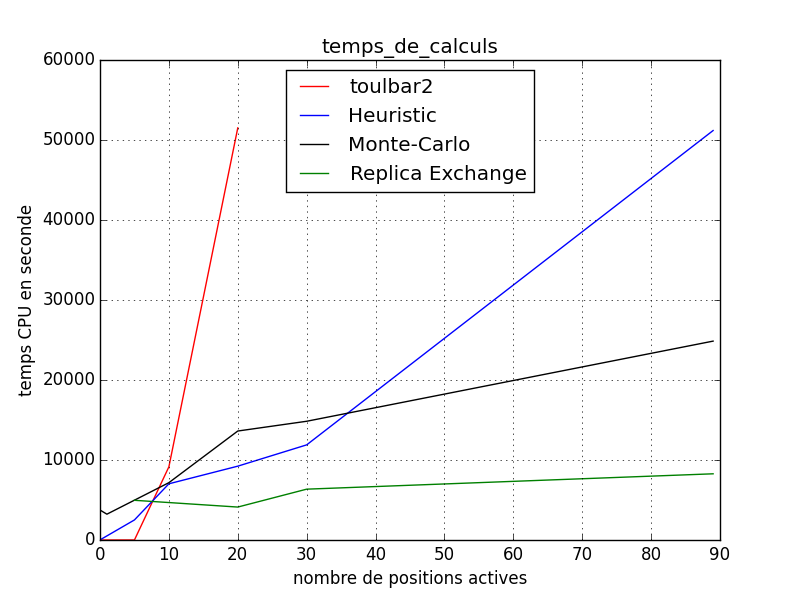
\includegraphics[width=12cm]{temps_de_calculs.png} &
      \end{tabular}
      
      \caption{Temps d'occupation du processeur selon le nombre de positions actives.}
\label{graph:temps_CPU}
    \end{figure}
    
    
    \clearpage
    \section{Les tests} 
   \subsection{Tous les résidus actifs} 


   \subsubsection{Les meilleures énergies} 

    \begin{table}[h]
      \centering

      \begin{tabular}{cccccccccc}

        \toprule
        Protéine & h & MC3 & MC43 & RE1 & RE2 & RE5 & RE3 & RE32 & RE4 \\
        \cmidrule{1-10}
        1A81 & -521 & -538 & -522 & -525 & -520 & -520 & -514 & -512 & -518 \\
        1ABO & -272 & -274 & -268 & -273 & -269 & -273 & -268 & -271 & -272 \\
        1BM2 & -484 & -500 & -486 & -488 & -481 & -489 & -478 & -476 & -486 \\
        1CKA & -252 & -258 & -249 & -259 & -251 & -251 & -247 & -246 & -249 \\
        1G9O & -428 & -435 & -428 & -429 & -421 & -430 & -428 & -425 & -428 \\
        1M61 & -480 & -493 & -479 & -483 & -480 & -481 & -480 & -480 & -480 \\
        1O4C & -535 & -545 & -531 & -536 & -529 & -536 & -527 & -524 & -532 \\
        1R6J & -407 & -419 & -414 & -415 & -409 & -411 & -409 & -408 & -414 \\
        2BYG & -457 & -469 & -454 & -461 & -456 & -460 & -456 & -454 & -462 \\
  
        \bottomrule

      \end{tabular}      
      \caption{les meilleures énergies pour tous les résidus actifs}
\label{tab:best_ener_all_all}      
    \end{table}


   \begin{figure}[t]
     \centering
     \begin{tabular}{cc}
       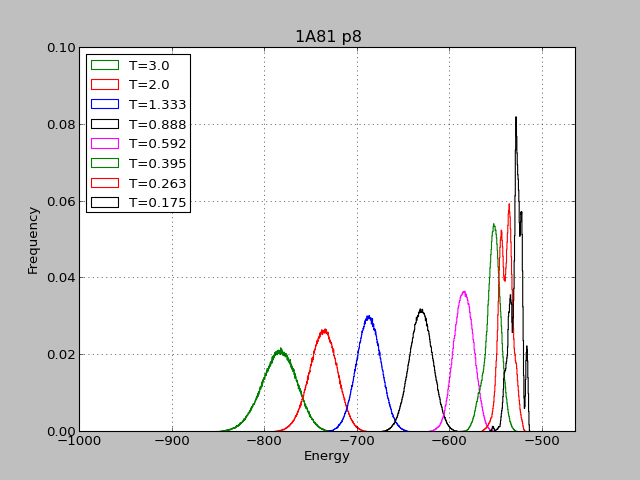
\includegraphics[width=12cm]{1A81_casa-p8.png} &
     \end{tabular}
     
     \caption{Distribution des énergies selon la température (protocole RE3).}
\label{graph:Distrib_E_T}
   \end{figure}


   \begin{figure}[t]
     \centering
     \begin{tabular}{cc}
       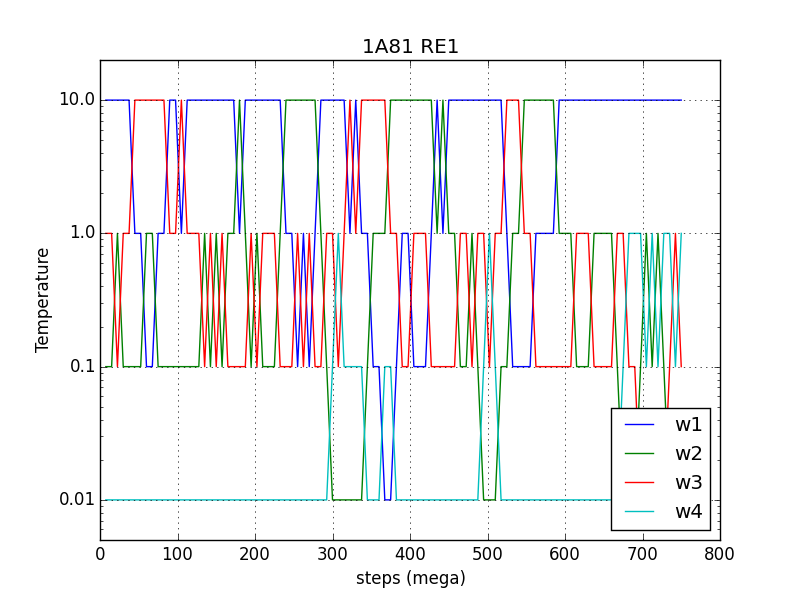
\includegraphics[width=8.45cm]{1A81-RE1-T_traj.png} &
       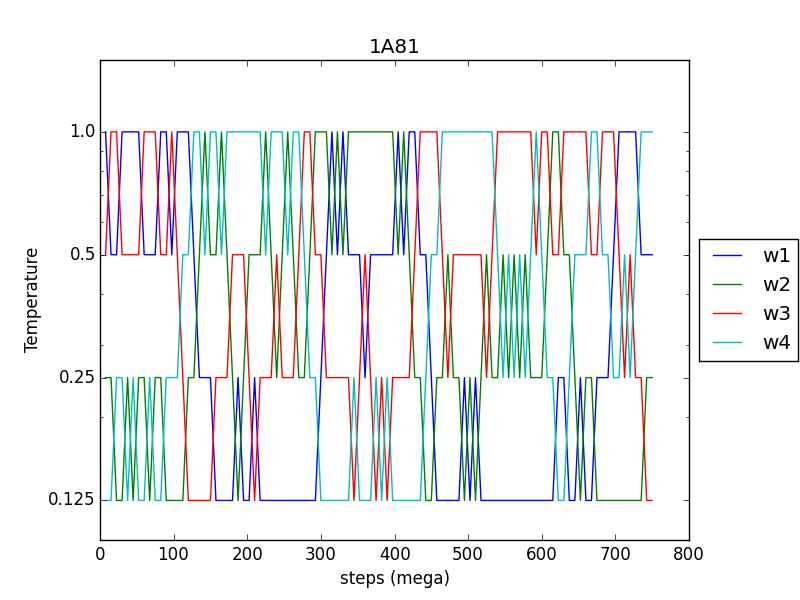
\includegraphics[width=8.45cm]{1A81-RE2-T_traj.png} \\
       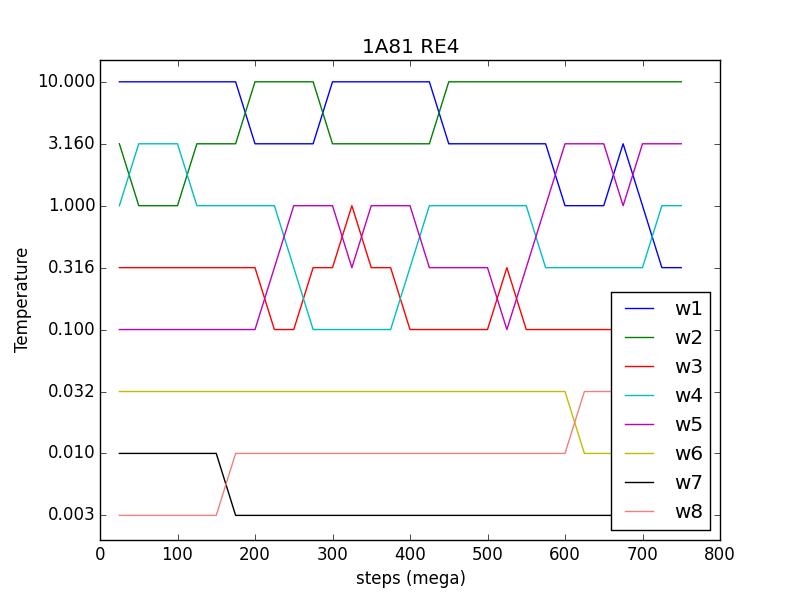
\includegraphics[width=8.45cm]{1A81-RE4-T_traj.png} &
       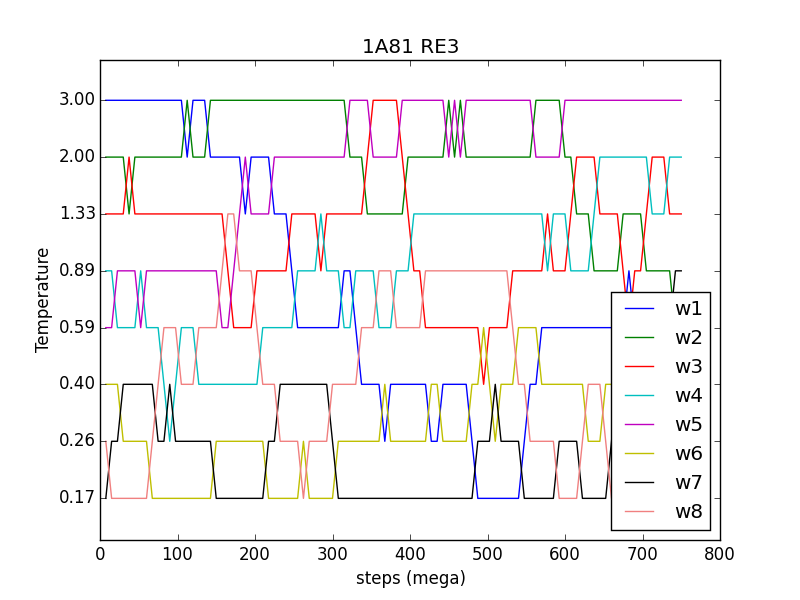
\includegraphics[width=8.45cm]{1A81-RE3-T_traj.png} \\
     \end{tabular}
     \caption{Variation de la température au court de la trajectoire de chaque marcheur (protocole RE1).}
\label{graph:TRAJ_T}
   \end{figure}

    \clearpage

   \begin{figure}[t]
     \centering
     \begin{tabular}{cc}
       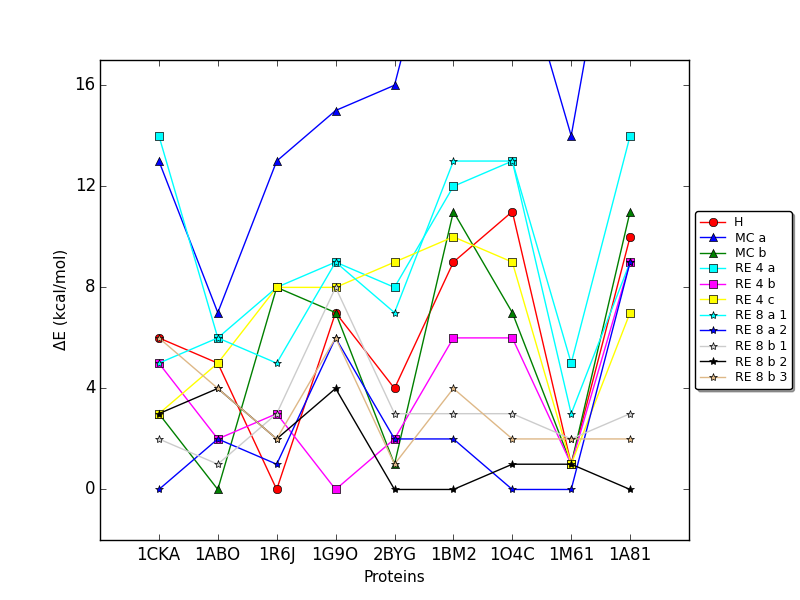
\includegraphics[width=18cm]{best_all.png} \\
     \end{tabular}
     \caption{Tous les protocoles.}
\label{graph:best_ener_all_all}
   \end{figure}


    \clearpage


   \begin{figure}[t]
     \centering
     \begin{tabular}{cc}
       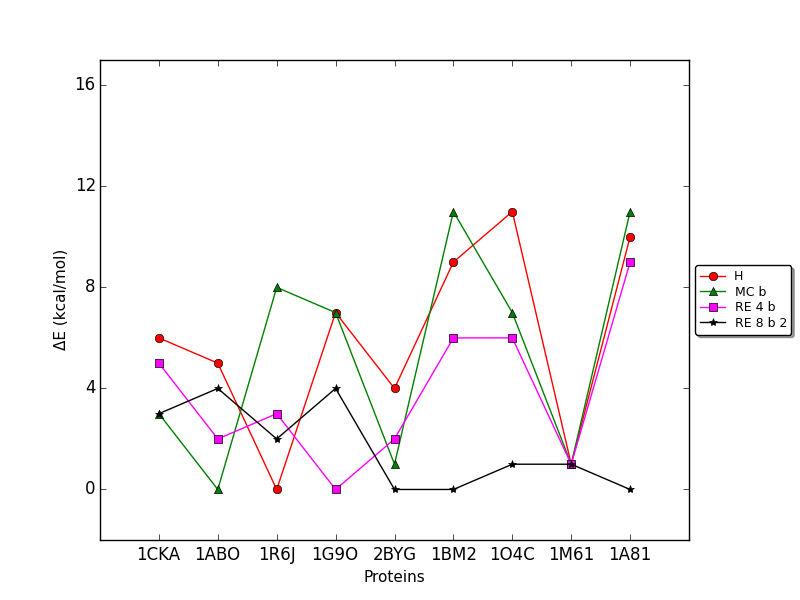
\includegraphics[width=8cm]{best_by_cat.png} &
       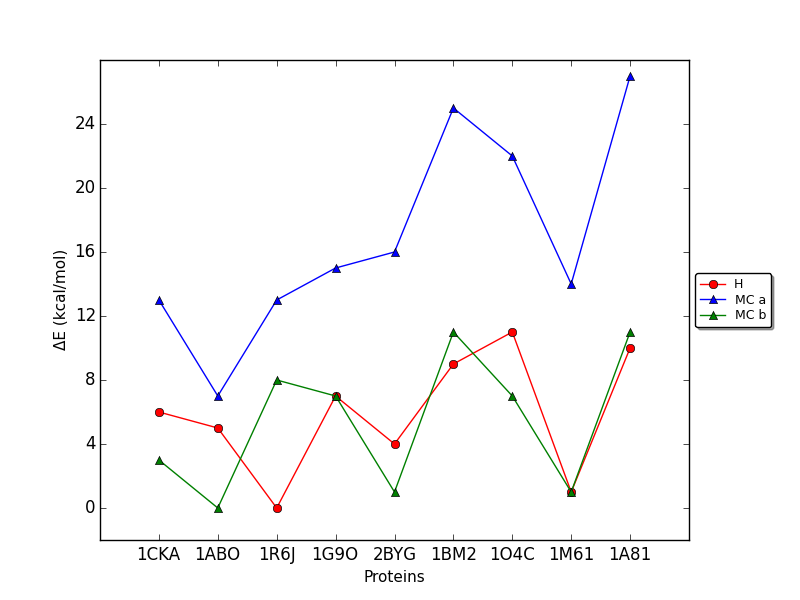
\includegraphics[width=8cm]{best_MC+H.png} \\
       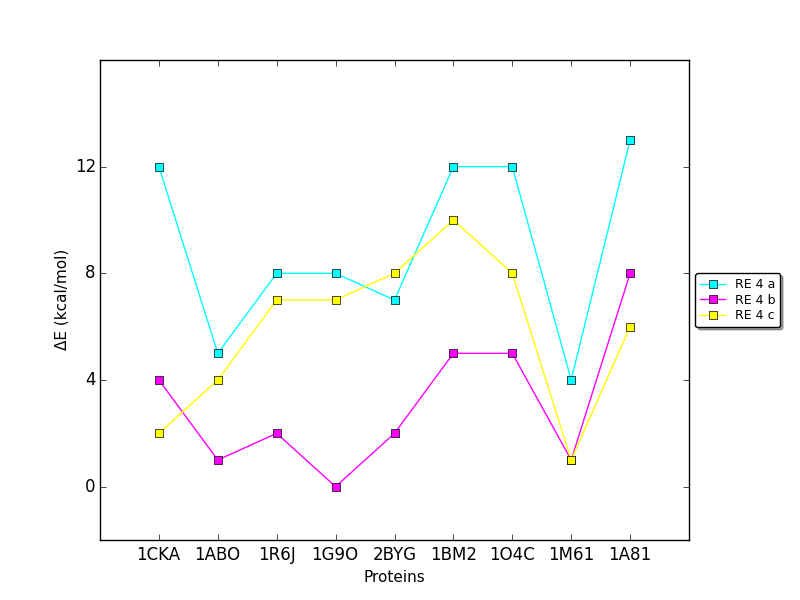
\includegraphics[width=8cm]{best_RE4.png} &
       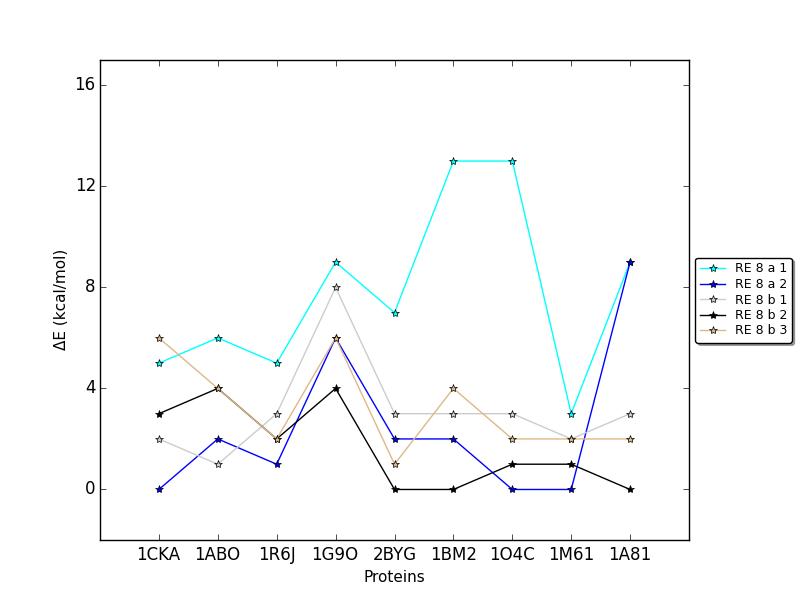
\includegraphics[width=8cm]{best_RE8.png} \\
     \end{tabular}
     \caption{Variation de la température au court de la trajectoire de chaque marcheur (protocole RE1).}
\label{graph:best_ener_by_algo}
   \end{figure}


    \clearpage

   \subsection{Tous les résidus inactifs}
 
   \subsubsection{Séquence native}

 
    \begin{table}[h]
      \centering

      \begin{tabular}{ccccccc}

        \toprule
        Protéine & GMEC & H- & MC0 & MC4- \\
        \cmidrule{1-5}
        1A81 & -585.1365 & 0 & -0.2547 & 0 \\
        1ABO & -320.1798 & 0 & 0 & 0 \\
        1BM2 & -553.5532 & 0 & -0.0564 & -0.0121 \\
        1CKA & -319.2787 & 0 & 0 & 0 \\
        1G9O & -481.1175 & 0 & -0.1394 & 0 \\
        1M61 & -555.9140 & 0 & 0 & 0 \\
        1O4C & -591.2115 & 0 & 0 & -0.1250 \\
        1R6J & -454.9340 & 0 & 0 & 0 \\
        2BYG & -507.0165 & 0 & 0 & 0 \\        
        \bottomrule


      \end{tabular}      
      \caption{L’énergie du GMEC et la différence avec les autres protocoles. Tous les résidus inactifs ()}
\label{tab:result_no_active}      
    \end{table}


   \subsubsection{Une position active}


    \begin{table}[h]
      \centering

      \begin{tabular}{ccc}


        \toprule
        Position & GMEC & MC4- \\
        \cmidrule{1-3}
        14 & -584.4693 & -0.0405 \\
        39 & -584.7378 & -0.0111 \\
        55 & -584.0477 & -0.0012 \\
        60 & -583.7763 & -0.0140 \\
        66 & -592.3835 & -0.0347 \\
        70 & -583.8950 & -0.0348 \\
        71 & -588.5916 & -0.0247 \\
        76 & -583.3815 & -0.0248 \\
        79 & -582.8485 & -0.0406 \\
        86 & -584.1412 & -0.0248 \\
        101 & -583.8406 & -0.0248 \\
        105 & -583.0197 & -0.0248 \\
        107 & -582.2241 & -0.0248 \\

        \bottomrule

      \end{tabular}      
      \caption{Liste des échecs pour 1A81}
\label{tab:result_1_active_1A81}      
    \end{table}


    \begin{table}[h]
      \centering

      \begin{tabular}{ccc}


        \toprule
        Position & GMEC & MC4- \\
        \cmidrule{1-3}
        2 & -553.3134 & -0.0040 \\
        3 & -553.5532 & -0.0121 \\
        5 & -553.0932 & -0.0179 \\
        6 & -553.5532 & -0.0121 \\
        8 & -556.1917 & -0.0148 \\
        10 & -551.4990 & -0.0149 \\
        11 & -551.8859 & -0.0149 \\
        12 & -550.8152 & -0.0148 \\
        13 & -553.4829 & -0.0451 \\
        14 & -553.5532 & -0.0121 \\
        15 & -553.5532 & -0.0121 \\
        17 & -553.5532 & -0.0121 \\
        18 & -553.0880 & -0.0121 \\
        19 & -553.5532 & -0.0270 \\
        20 & -553.0003 & -0.0121 \\
        21 & -553.5532 & -0.0121 \\
        22 & -553.1769 & -0.0121 \\
        29 & -553.5532 & -0.0121 \\
        34 & -553.5532 & -0.0270 \\
        36 & -555.3358 & -0.0317 \\
        37 & -553.5532 & -0.0121 \\
        41 & -553.5076 & -0.0121 \\
        46 & -552.9056 & -0.0149 \\
        49 & -553.5532 & -0.0121 \\
        51 & -553.5532 & -0.0179 \\
        55 & -551.8384 & -0.0121 \\
        56 & -553.5532 & -0.0121 \\
        57 & -561.0695 & -0.0121 \\
        58 & -553.5532 & -0.0121 \\
        62 & -553.5532 & -0.0121 \\
        65 & -553.5532 & -0.0121 \\
        66 & -551.2026 & -0.0179 \\
        68 & -552.6182 & -0.0148 \\
        70 & -553.5532 & -0.0121 \\
        72 & -552.2724 & -0.0121 \\
        73 & -553.5532 & -0.0121 \\
        75 & -553.5532 & -0.0179 \\
        77 & -553.0234 & -0.0466 \\
        80 & -553.5532 & -0.0121 \\
        81 & -553.5532 & -0.0121 \\
        82 & -548.0641 & -0.0121 \\
        83 & -553.5532 & -0.0121 \\
        85 & -550.1884 & -0.0122 \\
        86 & -552.7375 & -0.0148 \\
        87 & -550.6139 & -0.0121 \\
        90 & -552.8601 & -0.0009 \\
        91 & -553.5532 & -0.0121 \\
        92 & -553.5532 & -0.0121 \\
        93 & -553.2772 & -0.0148 \\
        94 & -553.3207 & -0.0251 \\
        96 & -553.5532 & -0.0121 \\
        \bottomrule

      \end{tabular}      
      \caption{Liste des échecs pour 1BM2}
\label{tab:result_1_active_1BM2}      
    \end{table}




    \begin{table}[h]
      \centering

      \begin{tabular}{ccc}


        \toprule
        Position & GMEC & MC4- \\
        \cmidrule{1-3}
        17 & -316.1693 & -0.0109 \\

        \bottomrule
      \end{tabular}      
      \caption{Liste des échecs pour 1CKA}
\label{tab:result_1_active_1CKA}      
    \end{table}

    \begin{table}[h]
      \centering

      \begin{tabular}{ccc}

        \toprule
        Position & GMEC & MC4 \\
        \cmidrule{1-3}
        58 & -561.9469 & -0.0138 \\
       \bottomrule        
      \end{tabular}      
      \caption{Liste des échecs pour 1M61}
\label{tab:result_1_active_1M61}      
    \end{table}
    

    \begin{table}[h]
      \centering
      
      \begin{tabular}{ccc}
        
        \toprule
        Position & GMEC & MC4- \\
        \cmidrule{1-3}
        1 & -591.2115 & -0.1380 \\
        2 & -591.2115 & -0.1250 \\
        3 & -591.2115 & -0.1250 \\
        4 & -590.7216 & -0.0319 \\
        5 & -590.5458 & -0.1071 \\
        6 & -591.2115 & -0.1521 \\
        7 & -590.7923 & -0.1429 \\
        8 & -591.2115 & -0.1250 \\
        9 & -591.2115 & -0.1728 \\
        10 & -591.2115 & -0.2572 \\
        11 & -589.9443 & -0.2489 \\
        12 & -591.1022 & -0.1137 \\
        13 & -589.9867 & -0.0535 \\
        14 & -591.2115 & -0.1250 \\
        15 & -589.4899 & -0.0436 \\
        16 & -591.2115 & -0.1521 \\
        17 & -590.4460 & -0.0557 \\
        18 & -589.0053 & -0.1366 \\
        19 & -590.7580 & -0.0348 \\
        20 & -591.2115 & -0.1250 \\
        21 & -591.2115 & -0.1600 \\
        22 & -591.2115 & -0.1250 \\
        23 & -590.5249 & -0.1530 \\
        24 & -590.7262 & -0.0630 \\
        25 & -591.2115 & -0.1250 \\
        26 & -591.2115 & -0.1250 \\
        27 & -590.8058 & -0.1194 \\
        28 & -591.2115 & -0.1250 \\
        29 & -591.2115 & -0.1571 \\
        30 & -590.5207 & -0.0221 \\
        31 & -590.5507 & -0.0530 \\
        32 & -591.2115 & -0.1571 \\
        33 & -591.2115 & -0.1234 \\
        34 & -590.7486 & -0.1258 \\
        35 & -591.2115 & -0.0378 \\
        36 & -589.1510 & -0.0974 \\
        37 & -591.0133 & -0.0941 \\
        38 & -589.2126 & -0.2743 \\
        39 & -589.0387 & -0.1890 \\
        40 & -590.8793 & -0.0883 \\
        41 & -589.4209 & -0.0409 \\
        42 & -591.2115 & -0.1250 \\
        43 & -587.9420 & -0.1315 \\
        44 & -589.8470 & -0.0595 \\
        45 & -591.2115 & -0.1712 \\
        46 & -588.8346 & -0.2668 \\
        47 & -589.9117 & -0.2773 \\
        48 & -588.6520 & -0.2625 \\
        49 & -591.2115 & -0.2120 \\
        50 & -590.6561 & -0.0807 \\
        51 & -591.1249 & -0.2986 \\
        52 & -589.7127 & -0.2734 \\
        53 & -590.7224 & -0.3012 \\
        54 & -590.8735 & -0.3615 \\
        55 & -588.6242 & -0.2007 \\
        56 & -591.2115 & -0.2120 \\
        57 & -591.2115 & -0.1250 \\
        58 & -590.6832 & -0.0743 \\
        59 & -591.2115 & -0.0378 \\
        60 & -591.1842 & -0.1082 \\
        61 & -590.6996 & -0.1272 \\
        62 & -595.8620 & -0.0899  \\
        63 & -591.2115 & -0.0974 \\
        64 & -588.8836 & -0.1014 \\
        65 & -591.2115 & -0.1571 \\
        66 & -590.1420 & -0.1533 \\
        67 & -587.5415 & -0.0433 \\
        68 & -590.1771 & -0.1541 \\
        69 & -591.2115 & -0.1250 \\
        70 & -590.4684 & -0.1066 \\
        71 & -591.2115 & -0.1250 \\
        72 & -591.2115 & -0.1311 \\
        73 & -591.2115 & -0.1250 \\
        74 & -588.7096 & -0.1169 \\
        75 & -590.2437 & -0.0505 \\
        76 & -591.2115 & -0.1521 \\
        78 & -587.6940 & -0.0821 \\
        79 & -589.9770 & -0.1380 \\
        80 & -591.1165 & -0.0661 \\
        81 & -590.2528 & -0.1229 \\
        82 & -589.8459 & -0.0724 \\
        83 & -590.2079 & -0.0513 \\
        84 & -591.2095 & -0.0433 \\
        85 & -590.8011 & -0.1154 \\
        87 & -590.7787 & -0.0744 \\
        88 & -590.2860 & -0.0857 \\
        89 & -591.2115 & -0.1250 \\
        90 & -590.2493 & -0.1084 \\
        91 & -589.5602 & -0.0694 \\
        92 & -589.3260 & -0.1838 \\
        93 & -590.4697 & -0.0188 \\
        94 & -587.4192 & -0.3392 \\
        95 & -590.0201 & -0.2937 \\
        96 & -590.6312 & -0.2723 \\
        97 & -595.0049 & -0.2864 \\
        98 & -590.0135 & -0.2013 \\
        99 & -589.7855 & -0.2932 \\
        100 & -591.2115 & -0.2120 \\
        101 & -591.2115 & -0.2120 \\
        102 & -591.2115 & -0.2572 \\
        103 & -595.4168 & -0.1277 \\
        104 & -589.9208 & -0.3581 \\
        \bottomrule
       


      \end{tabular}      
      \caption{Liste des échecs pour 1O4C}
\label{tab:result_1_active_1O4C}
    \end{table}

    \begin{table}[h]
      \centering

      \begin{tabular}{ccc}


        \toprule
        Position & GMEC & MC4- \\
        \cmidrule{1-3}
         4 & -453.4484 & -0.0155  \\
        20 & -452.6464 & -0.0114 \\
        32 & -454.9340 & -0.0092 \\
        68 & -454.4856 & -0.0060 \\
        73 & -454.7809 & -0.0155 \\
        77 & -454.1344 & -0.0155 \\
        79 & -453.4729 & -0.0155 \\
        \bottomrule
      \end{tabular}      
      \caption{Liste des échecs pour 1R6J }
\label{tab:result_1_active_1R6J}
    \end{table}

    \begin{table}[h]
      \centering

      \begin{tabular}{ccc}

        \toprule
        Position & GMEC & MC4- \\
        \cmidrule{1-3}
        1 & -505.2910 & -0.0132 \\
        3 & -506.7960 & -0.0254 \\
        4 & -505.5800 & -0.0023 \\
        5 & -506.8732 & -0.0948 \\
        49 & -505.5183 & -0.0135 \\
        59 & -507.0165 & -0.0100 \\
        85 & -506.6217 & -0.0101 \\
        88 & -505.2286 & -0.0097 \\
        95 & -506.3195 & -0.0131 \\
        \bottomrule
      \end{tabular}      
      \caption{Liste des échecs pour 2BYG }
\label{tab:result_1_active_2BYG}
    \end{table}


   \subsubsection{Cinq positions actives}


    \begin{table}[h]
      \centering

      \begin{tabular}{ccccc}


        
        \toprule
        Protéine & GMEC & H & MC4 & RE3 \\
        \cmidrule{1-5}
        1A81 1 & -579.3989 & 0 & 0 &  \\
        1A81 2 & -575.2254 & 0 & 0 &  \\
        1A81 3 & -582.7452 & 0 & 0 &  \\
        1A81 4 & -569.9383 & 0 & -5.3443 & 0 \\
        1A81 5 & -591.8143 & 0 & 0 &  \\
        1ABO 1 & -315.4497 & 0 & 0 &  \\
        1ABO 2 & -316.6637 & 0 & 0 &  \\
        1ABO 3 & -307.4824 & 0 & 0 &  \\
        1ABO 4 & -313.7710 & 0 & 0 &  \\
        1ABO 5 & -313.5695 & 0 & 0 &  \\
        1BM2 1 & -548.2341 & 0 & 0 &  \\
        1BM2 2 & -554.8135 & 0 & 0 &  \\
        1BM2 3 & -557.8629 & 0 & 0 &  \\
        1BM2 4 & -544.9791 & 0 & 0 &  \\
        1BM2 5 & -550.2956 & 0 & -0.0121 &  \\
        1CKA 1 & -315.0859 & 0 & 0 &  \\
        1CKA 2 & -309.7692 & 0 & 0 &  \\
        1CKA 3 & -317.3820 & 0 & 0 &  \\
        1CKA 4 & -314.8550 & 0 & 0 &  \\
        1CKA 5 & -312.0405 & -0.0001 & -0.0001 &  \\
        1G9O 1 & -469.9540 & 0 & 0 &  \\
        1G9O 2 & -476.4094 & 0 & 0 &  \\
        1G9O 3 & -479.7190 & 0 & 0 &  \\
        1G9O 4 & -478.9513 & 0 & 0 &  \\
        1G9O 5 & -480.7260 & 0 & 0 &  \\
        1M61 1 & -557.6647 & 0 & 0 &  \\
        1M61 2 & -546.9587 & 0 & 0 &  \\
        1M61 3 & -553.0731 & 0 & 0 &  \\
        1M61 4 & -555.0885 & 0 & 0 &  \\
        1M61 5 & -554.6356 & 0 & 0 &  \\
        1O4C 1 & -584.4267 & 0 & -0.0655 &  \\
        1O4C 2 & -584.8989 & 0 & -0.1437 &  \\
        1O4C 3 & -588.4971 & 0 & -0.1164 &  \\
        1O4C 4 & -587.7129 & 0 & -0.1400 &  \\
        1O4C 5 & -587.6514 & 0 & -0.1168 &  \\
        1R6J 1 & -444.5018 & 0 & 0 &  \\
        1R6J 2 & -449.3043 & 0 & -0.9421 & 0 \\
        1R6J 3 & -453.1139 & 0 & 0 &  \\
        1R6J 4 & -453.1139 & 0 & 0 &  \\
        1R6J 5 & -454.9340 & 0 & 0 &  \\
        2BYG 1 & -500.7946 & 0 & -0.0150 &  \\
        2BYG 2 & -506.2319 & 0 & 0 &  \\
        2BYG 3 & -506.8744 & 0 & -0.0131 &  \\
        2BYG 4 & -504.5135 & 0 & 0 &  \\
        2BYG 5 & -506.0052 & 0 & 0 &  \\
        \bottomrule
      \end{tabular}      
 \caption{Résultats 5 position actives}
\label{tab:result_5_actives}
\end{table}

   \subsubsection{Dix positions actives}


    \begin{table}[h]
      \centering

      \begin{tabular}{cccccc}


        \toprule
        Protéine & GMEC & toulbar2 & H & MC & RE \\
        \cmidrule{1-6}
        1A81 1 & yes & -583.9354 & 0. & 0. & \\
        1A81 2 & yes & -581.7802 & 0. & 0. & \\
        1A81 3 & yes & -587.4392 & -0.0001 & -0.1595 & \\
        1A81 4 & yes & -589.1322 & 0. & -0.0317 & \\
        1A81 5 & yes & -578.2558 & 0. & -0.0563 & \\
        1ABO 1 & yes & -309.1670 & -0.0675 & -0.9054 & \\
        1ABO 2 & yes & -308.8387 & 0. & 0. & \\
        1ABO 3 & yes & -303.8520 & 0. & 0. & \\
        1ABO 4 & yes & -310.0087 & 0. & -0.0128 & \\
        1ABO 5 & yes & -301.6727 & 0. & 0. & \\
        1BM2 1 & yes & -549.8638 & 0. & -0.0950. & \\
        1BM2 2 & yes & -541.5944 & 0. & 0. & \\
        1BM2 3 & yes & -543.7434 & 0. & 0. & \\
        1BM2 4 & yes & -549.0453 & 0. & 0. & \\
        1BM2 5 & yes & -544.1447 & 0. & -0.1082 & \\
        1CKA 1 & yes & -305.8477 & 0. & 0. & \\
        1CKA 2 & yes & -309.9886 & 0. & 0. & \\
        1CKA 3 & yes & -304.6618 & 0. & 0. & \\
        1CKA 4 & yes & -302.4894 & 0. & 0. & \\
        1CKA 5 & yes & -299.2329 & -0.2859 & -3.2525 & 0. \\
        1G9O 1 & yes & -466.6764 & 0. & 0. & \\
        1G9O 2 & yes & -478.8797 & 0. & 0. & \\
        1G9O 3 & yes & -477.2503 & -0.1366 & 0. & \\
        1G9O 4 & yes & -470.6458 & 0. & 0. & \\
        1G9O 5 & yes & -464.8659 & 0. & -3.9599 & 0.\\
        1M61 1 & yes & -550.0699 & 0. & -0.0776 & \\
        1M61 2 & yes & -538.6026 & -3.5105 & -4.5062 & 0.3215 \\
        1M61 3 & yes & -552.2673 & 0. & 0. & \\
        1M61 4 & yes & -550.0553 & 0. & 0. & \\
        1M61 5 & yes & -553.6559 & 0. & -0.0432 & \\
        1O4C 1 & yes & -587.4665 & 0. & -0.1121 & \\
        1O4C 2 & yes & -585.8545 & 0. & -0.1046 & \\
        1O4C 3 & yes & -580.3505 & 0. & -0.1519 & \\
        1O4C 4 & yes & -587.1548 & 0. & -0.1545 & \\
        1O4C 5 & yes & -590.2650 & 0. & -0.1753 & \\
        1R6J 1 & yes & -448.8351 & 0. & -2.4022 & -2.3986 \\
        1R6J 2 & yes & -448.4631 & 0. & -1.0398 & \\
        1R6J 3 & yes & -450.3950 & 0. & -0.0106 & \\
        1R6J 4 & yes & -451.7211 & 0. & 0. & \\
        1R6J 5 & yes & -450.9943 & 0. & -0.0162 & \\
        2BYG 1 & no  & -5.7485   & -505.6397 & -0.0337 & \\
        2BYG 2 & yes & -504.7389 & 0. & 0. & \\
        2BYG 3 & yes & -504.3048 & 0. & -0.0833 & \\
        2BYG 4 & yes & -504.3466 & 0. & -0.2149 & \\
        2BYG 5 & yes & -491.6095 & 0. & 0. & \\
        
        \bottomrule


 \end{tabular}      
 \caption{Résultats 10 positions actives }
\label{tab:result_10_actives}
\end{table}

   \subsubsection{Dix positions actives, mutations}


    \begin{table}[h]
      \centering

      \begin{tabular}{ccc}

        \toprule
        Protéine & H mut nb & MC mut nb \\
        \cmidrule{1-3}
        1A81 1 & 0  & 0 \\    
        1A81 2 & 0  & 0 \\
        1A81 3 & 0  & 2 \\
        1A81 4 & 0  & 0 \\
        1A81 5 & 0  & 0 \\
        1ABO 1 & 0  & 4 \\ 
        1ABO 2 & 0  & 0 \\
        1ABO 3 & 0  & 1 \\
        1ABO 4 & 2  & 2 \\
        1ABO 5 & 0  & 0 \\
        1BM2 1 & 0  & 2 \\
        1BM2 2 & 0  & 0 \\
        1BM2 3 & 0  & 0 \\
        1BM2 4 & 0  & 1 \\
        1BM2 5 & 0  & 2 \\
        1CKA 1 & 0  & 0 \\
        1CKA 2 & 0  & 1 \\
        1CKA 3 & 0  & 0 \\
        1CKA 4 & 0  & 0 \\
        1CKA 5 & 5  & 3 \\
        1G9O 1 & 0  & 0 \\
        1G9O 2 & 0  & 0 \\
        1G9O 3 & 0  & 0 \\
        1G9O 4 & 0  & 0 \\
        1G9O 5 & 0  & 3 \\
        1M61 1 & 0  & 2 \\
        1M61 2 & 3  & 7 \\
        1M61 3 & 0  & 0 \\
        1M61 4 & 0  & 0 \\
        1M61 5 & 0  & 0 \\
        1O4C 1 & 0  & 0 \\
        1O4C 2 & 0  & 0 \\
        1O4C 3 & 0  & 0 \\
        1O4C 4 & 0  & 0 \\
        1O4C 5 & 0  & 3 \\
        1R6J 1 & 0  & 3 \\
        1R6J 2 & 0  & 2 \\
        1R6J 3 & 0  & 0 \\
        1R6J 4 & 0  & 0 \\
        1R6J 5 & 0  & 0 \\
        2BYG 1 & no & no \\ 
        2BYG 2 & 0  & 0 \\
        2BYG 3 & 0  & 1 \\
        2BYG 4 & 1  & 3 \\
        2BYG 5 & 0  & 0 \\        
        \bottomrule

 \end{tabular}      
 \caption{Mutations 10 positions actives }
\label{tab:mutations_10_actives}
\end{table}

   \subsubsection{Vingt et trente positions actives}


    \begin{table}[h]
      \centering

      \begin{tabular}{cccccc}


        \toprule
        Protéine & GMEC & toulbar2 & H & MC & RE \\
        \cmidrule{1-6}
        1A81 1 & yes  &  -566.9106 & 0. & -0.3275 & -0.3851 \\         
        1A81 2 & yes  &  -564.6618 & -0.1705 & -2.4355 & -1.0069 \\   
        1A81 3 & yes  &  -572.7774 & 0. & -0.4640 & -0.6186 \\         
        1A81 4 & yes  &  -572.9780 & -0.3878 & -0.5748 & -0.6991 \\    
        1A81 5 & yes  &  -572.7410 & -0.0068 & -0.5088 & -0.1541 \\    
        1ABO 1 & yes  &  -299.6592 & -0.1205 & -1.1159 & -0.2153 \\   
        1ABO 2 & no   &  -13.8563  & -298.3854 & 0. & 0. \\               
        1ABO 3 & no   &  -1.2190   & -298.3854 & 0. & 0. \\                 
        1ABO 4 & no   &  -1.9940   & -297.8545 & -0.0076 & 0. \\            
        1ABO 5 & no   &  -3.5418   & -297.8009 & -0.9483 & -0.9483 \\       
        1BM2 1 & yes  &  -526.0936 & 0. & -0.0619 & -0.1584 \\         
        1BM2 2 & no   &  -7.5304   & -525.3588 & -0.0725 & -0.0143 \\     
        1BM2 3 & yes  &  -534.3861 & -0.0229 & -0.4762 & -0.2897 \\    
        1BM2 4 & no   &  -0.1186   & -526.8307 & -2.5883 & -0.0789 \\     
        1BM2 5 & yes  &  -535.3334 & -0.2396 & -0.3746 & -0.3746 \\    
        1CKA 1 & yes  & -295.8571  & 0.& 0. & 0. \\                   
        1CKA 2 & yes  & -295.3571  & 0. & 0. & 0. \\                   
        1CKA 3 & yes  & -293.8687  & 0. & 0. & 0.\\                   
        1CKA 4 & no   &  -4.3122   & -293.8687 & 0. & 0. \\               
        1CKA 5 & no   &  -4.2849   & -293.4203 & 0. & 0. \\           
        1G9O 1 & no   &  -2.0574   & -451.4604 & -1.2525 & -1.2525 \\ 
        1G9O 2 & no   &  -3.2106   & -453.2474 & -0.2177 & -0.1915 \\ 
        1G9O 3 & no   &  -1.9008   & -453.7856 & -0.4417 & -0.1019 \\ 
        1G9O 4 & no   &  -0.5030   & -456.7331 & -0.3855 & -0.1455 \\ 
        1G9O 5 & no   &  -0.4298   & -456.9981 & -0.1495 & -0.5114 \\ 
        1M61 1 & yes  & -528.0700 & 0. & 0. & 0. \\               
        1M61 2 & yes  & -528.7653 & 0. & 0. & 0. \\               
        1M61 3 & yes  & -530.0684 & 0. & 0. & 0. \\               
        1M61 4 & yes  & -534.5248 & 0. & 0. & 0.\\               
        1M61 5 & yes  & -548.0096 & 0. & -0.2521 & -0.1345 \\     
        1O4C 1 & no   &  -574.0047 & -0.3465 & -0.0690 & -0.0587 \\    
        1O4C 2 & no   &  -6.4214   & -574.8584 & -0.1963 & -0.3175 \\         
        1O4C 3 & yes  & -573.6314 &  0. & -0.3461 & -0.0997 \\             
        1O4C 4 & yes  & -575.8667 &  0. & -0.3640 & -0.1382 \\             
        1O4C 5 & no   & -573.3479 &  0. & -0.1131 & -0.2206 \\      
        1R6J 1 & yes  & -440.7417 &  0. & -0.2604 & -0.2002 \\        
        1R6J 2 & yes  & -437.2537 &  0. & -0.0071 & -0.0183 \\        
        1R6J 3 & yes  & -439.4335 &  0. & -0.0537 & -0.0732 \\       
        1R6J 4 & yes  & -439.5988 &  0. & -0.0639 & -0.0601 \\        
        1R6J 5 & yes  & -438.0222 &  0. & -0.0735 & -0.0244 \\        
        2BYG 1 & yes  & -496.2991 &  0. & -3.1878 & -0.0257 \\        
        2BYG 2 & yes  & -494.8723 &  0. & -0.0524 & -0.0831 \\        
        2BYG 3 & yes  & -494.4390 &  0. & -1.3564 & -0.0826 \\        
        2BYG 4 & yes  & -495.9213 &  0. & -0.1968 & -0.6022 \\        
        2BYG 5 & no   &  -1.8604   & -497.5123 & -0.0933 & -0.0386 \\   
       \bottomrule


 \end{tabular}   
\label{tab:result_20_actives}   
\end{table}


\begin{table}[h]
      \centering

      \begin{tabular}{cccccc}


        \toprule
        Protéine & GMEC & toulbar2 & H & MC & RE \\
        \cmidrule{1-6}
        1A81 1 & no & -1.2074    &    -562.9572 & -0.6353 &  \\          
        1A81 2 & no & -2.5520    &    -570.2620 & -0.0578 & \\          
        1A81 3 & no & -43.5263   &    -562.9572 & -2.4996 & -1.2025 \\         
        1A81 4 & no & -5.1300    &    -559.6145 & -0.0305 & \\          
        1A81 5 & no & -3.2417    &    -553.1077 & -1.9586 & -0.5791\\         
        1ABO 1 & no & -44.5504   &    -296.5680 & 0. & \\                   
        1ABO 2 & no & -12.7303   &    -294.8500 & 0. & \\                   
        1ABO 3 & no & -9.3870    &    -295.2689 & -0.2630 & \\          
        1ABO 4 & no & -10.7691   &    -296.5680 & 0. & \\                   
        1ABO 5 & no & -4.3907    &    -296.5680 & 0. & \\                    
        1BM2 1 & no & -22.5876   &    -556.1168 & -1.7290 & -1.6013 \\         
        1BM2 2 & no & -22.1386   &    -556.7539 & -1.9856 & -1.5876 \\     
        1BM2 3 & no & -22.5410   &    -556.1168 & -1.9990 & -1.1541 \\
        1BM2 4 & no & -15.2639   &    -556.8507 & -2.2127 & -2.3854 \\         
        1BM2 5 & no & -15.9890   &    -556.3240 & -2.83542 & -1.1937 \\        
        1CKA 1 & no & -6.2700    &    -293.4203 & 0. & \\                    
        1CKA 2 & no & -2.0995    &    -293.4203 & 0. & \\                    
        1CKA 3 & no & -47.0217   &    -291.9243 & 0. & \\                   
        1CKA 4 & no & -44.0830   &    -293.4203 & 0. & \\                   
        1CKA 5 & no & -8.8608    &    -293.2709 & 0. & \\                    
        1G9O 1 & no & -2.0816    &    -449.0890 & -1.5942 & 0. \\               
        1G9O 2 & no & -0.3270    &    -452.6676 & -0.3126 & \\          
        1G9O 3 & no & -17.7150   &    -450.0341 & -1.5667 & -1.5667 \\         
        1G9O 4 & no & -2.9758    &    -453.9682 & -1.4284 & -1.6202 \\          
        1G9O 5 & no & -445.8910  &    -1.6890 & -7.6985 & -2.3857 \\          
        1M61 1 & no & -14.4935   &    -0.0097 & -523.9321 & 0. \\            
        1M61 2 & no & -5.0899    &    -531.3717 & -1.8749 & -0.0083 \\         
        1M61 3 & no & -3.5795    &    -527.2659 & -0.0154 & \\           
        1M61 4 & no & -16.1511   &    -530.2666 & 0. & \\              
        1M61 5 & no & -23.0927   &    -522.5696 & 0. & \\                 
        1O4C 1 & no & -14.9064   &    -571.4882 & -0.3435 & \\         
        1O4C 2 & no & -58.1558   &    -570.1458 & -0.0795 & \\         
        1O4C 3 & no & -9.9221    &    -569.9777 & -0.1789 & \\          
        1O4C 4 & no & -5.7790    &    -568.9839 & -0.0423 & \\          
        1O4C 5 & no & -9.9221    &    -569.9777 & -0.1789 & \\          
        1R6J 1 & yes& -435.4258  &     0.0 & -0.0246 & \\               
        1R6J 2 & no & -14.9800   &    -435.0087 & -0.0957 & \\         
        1R6J 3 & no & -439.8187  &    -439.8187 & -0.0440 & \\               
        1R6J 4 & no &  -435.0087  &    -0.0 & -0.0957 & \\               
        1R6J 5 & no & -435.0970  &    -0.7036 & -1.8823 & -0.0781 \\          
        2BYG 1 & no & -17.9752   &    -492.6879 & -0.1592 & \\         
        2BYG 2 & no & -0.3832    &    -492.3568 & -0.1502 & \\          
        2BYG 3 & no & -0.1442    &    -492.6879 & -0.1593 & \\          
        2BYG 4 & no & -492.6821 &    -0.0958 & -0.0050 & \\          
        2BYG 5 & no & -0.5003    &   -492.1595 & -0.6876 & \\           
       \bottomrule


 \end{tabular}      
\label{tab:result_echec_30}      
\end{table}

   \subsection{Etude au voisinnage de GMECs}


    \begin{table}[h]
      \centering

      \begin{tabular}{ccccc}


        \toprule
        Protein & GMEC & H & MC & RE \\
        \cmidrule{1-5}
        1CKA 3 & -304.6618 & 0 & 0 & \\
        1CKA 4 & -302.4894 & 0 & 0 & \\
        1CKA 5 & -299.2329 & -0.2859 & -3.2525 & 0 \\
        1G9O 3 & -477.2503 & -0.1366 & 0 & \\
        1G9O 4 & -470.6458 & 0 & 0 & \\
        1G9O 5 & -464.8659 & 0 & -3.9599 &  0 \\
        1M61 1 & -550.0699 & 0 & -0.0776 & \\
        1M61 2 & -538.6026 & -3.5105 & -4.5062 & 0.3215 \\
        1M61 5 & -553.6559 & 0 & -0.0432 & \\
        \bottomrule       
      \end{tabular}      
\label{tab:voisinnage_rappel}      
    \end{table}


    \begin{table}[h]
      \centering

      \begin{tabular}{ccccccc}


        \toprule
        Protein & seq-rot nb gmec+1 & H rank  & MC rank  & seq nb gmec+1 & H mut nb & MC mut nb \\
        \cmidrule{1-7}
        1CKA 3 & 67669 & 1 & 1 & 227 & 0 & 0 \\
        1CKA 4 & 4649 & 1 & 1 & 498 & 0 & 0 \\
        1CKA 5 & 1388 & 78 & ? & 77 & 0 & 2 \\
        1G9O 3 & 354559 & 23 & 1 & 63 & 1 & 0 \\
        1G9O 4 & 22639 & 1 & 1 & 381 & 0 & 0 \\
        1G9O 5 & 8658395 & 1 & ? &  11 & 0 & 3 \\
        1M61 1 & 11199153 & ? & ? & 21 & 3 & 7 \\
        1M61 2 & 11199153 & 1 & 1 & 88 & 0 & 0 \\
        1M61 5 & 16417604 & 1 & 1 & 83 & 0 & 0 \\
        \bottomrule
      \end{tabular} 
\label{tab:etude_au_voisinnage}           
\end{table}


    \clearpage
    
    \begin{figure}[h]
      \centering
      \begin{tabular}{c} 
        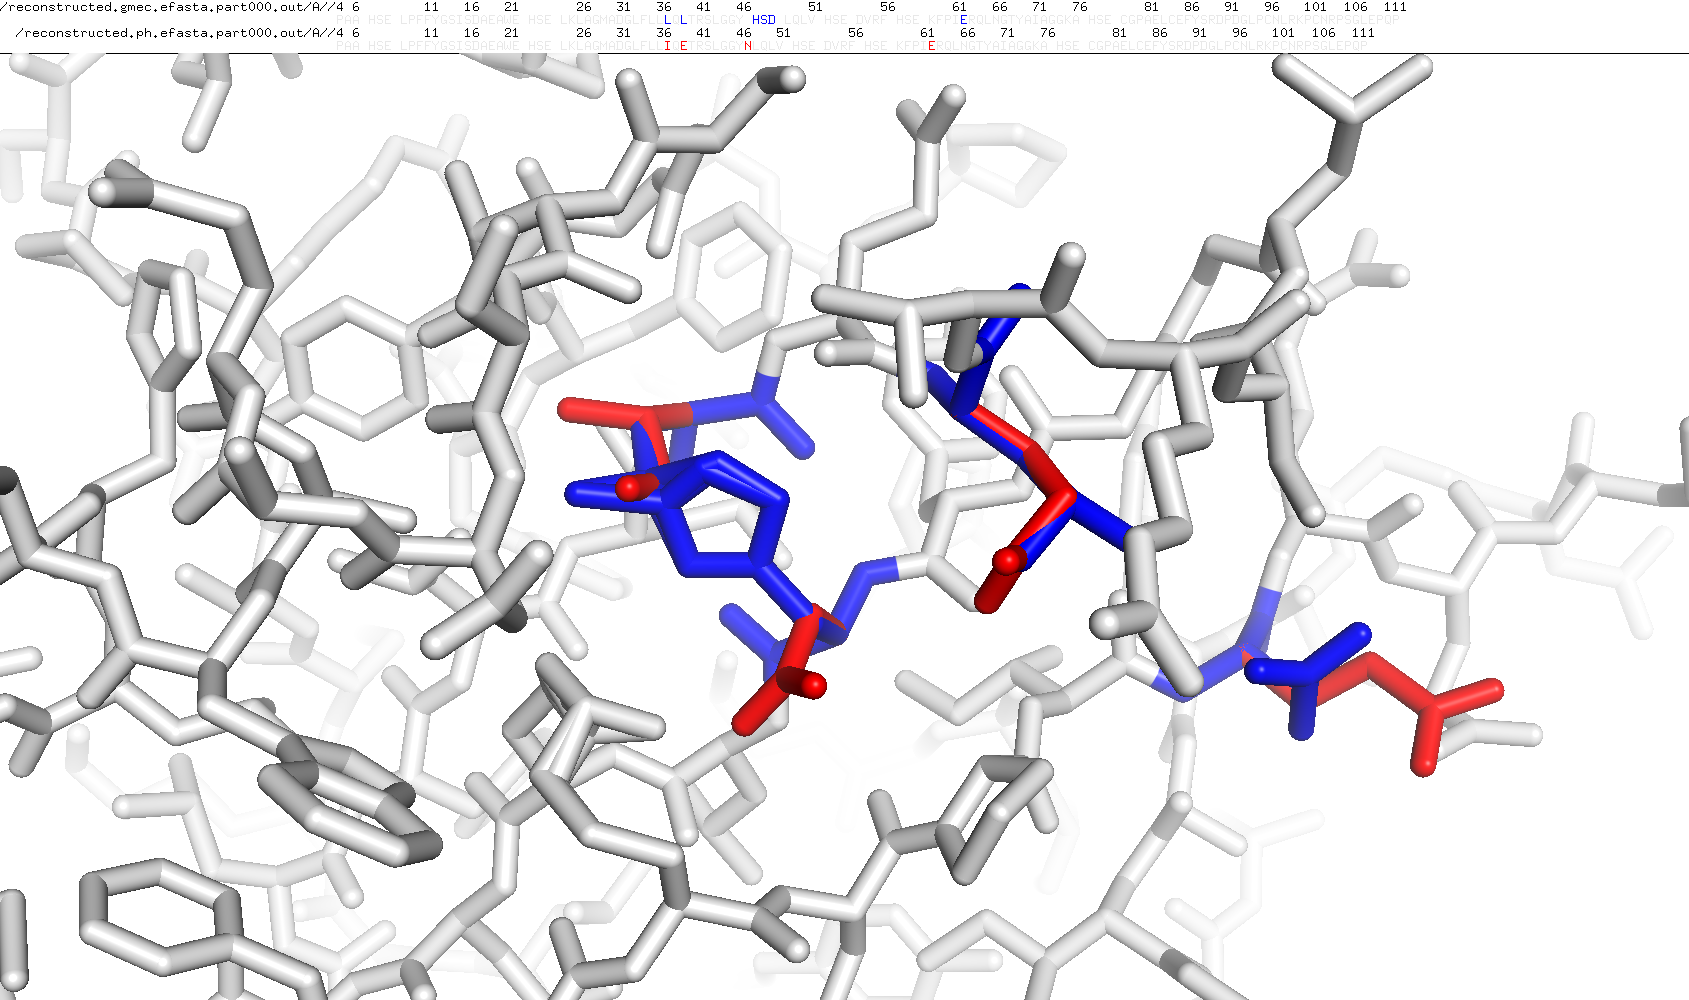
\includegraphics[width=14cm]{1M61_2_gmec_vs_ph.png} 
      \end{tabular}
      
      \caption{test: 1M61 2, GMEC vs H}
\label{image:1M61_2_GMEC_vs_H}
    \end{figure}
    
        
    \begin{figure}[h]
      \centering
      \begin{tabular}{c} 
        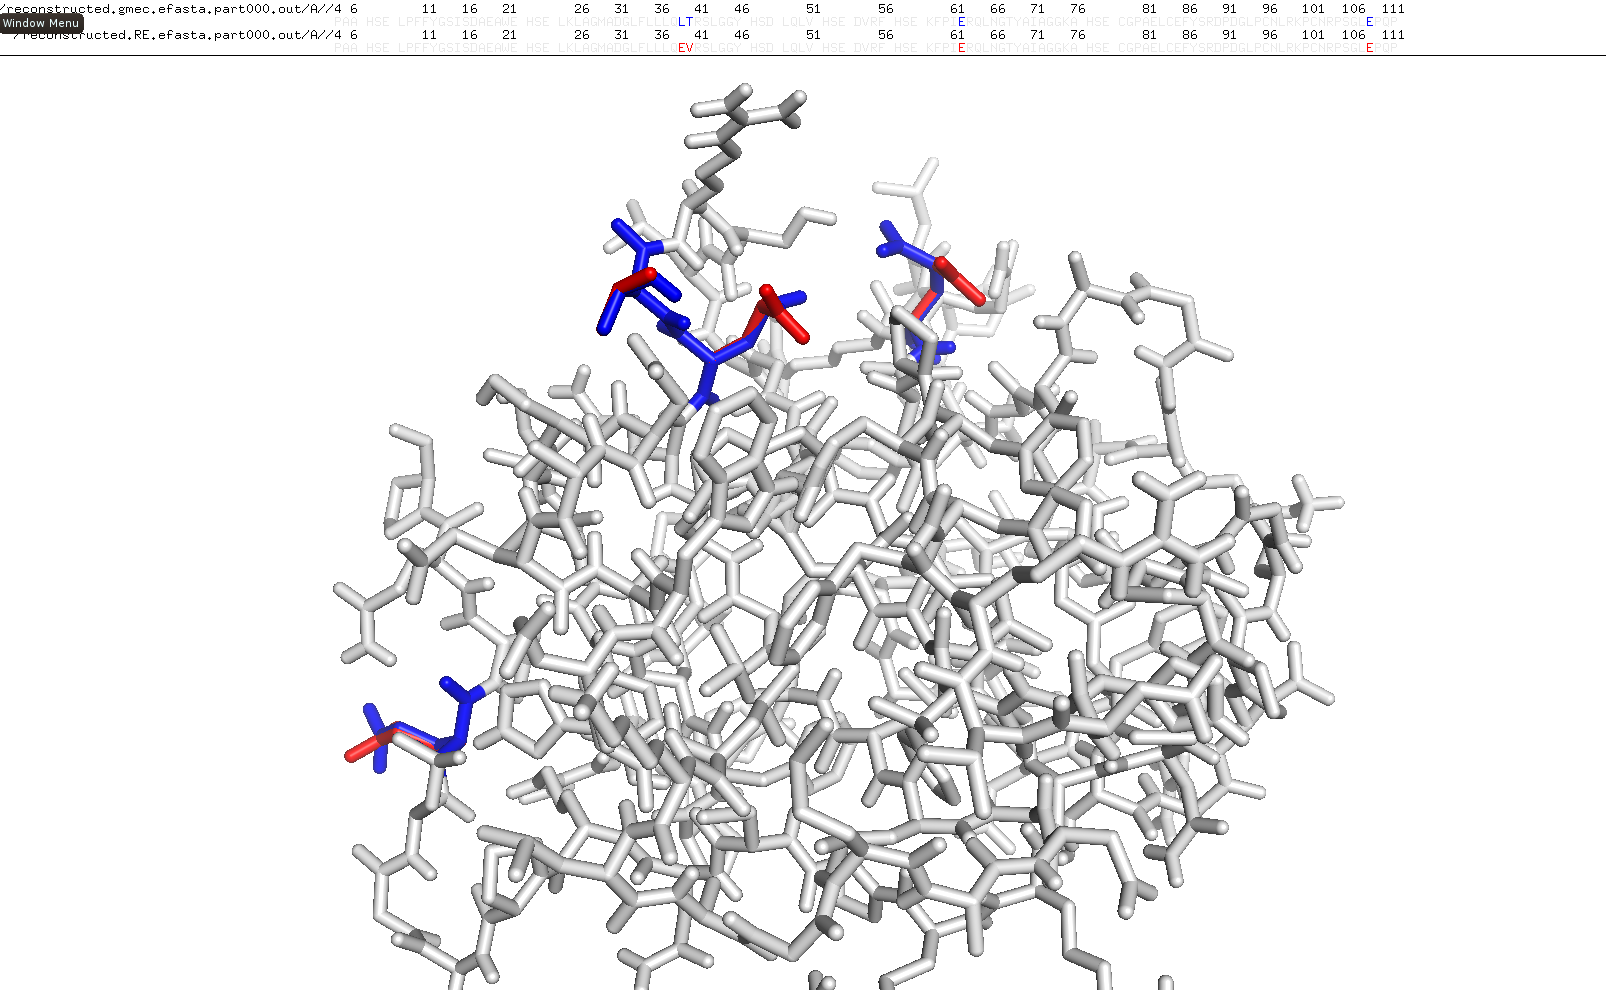
\includegraphics[width=14cm]{1M61_2_gmec_vs_RE.png} 
      \end{tabular}
      
      \caption{test: 1M61 2, GMEC vs RE}
\label{image:1M61_2_GMEC_vs_RE}
    \end{figure}
    
        
    \begin{figure}[h]
      \centering
      \begin{tabular}{c} 
        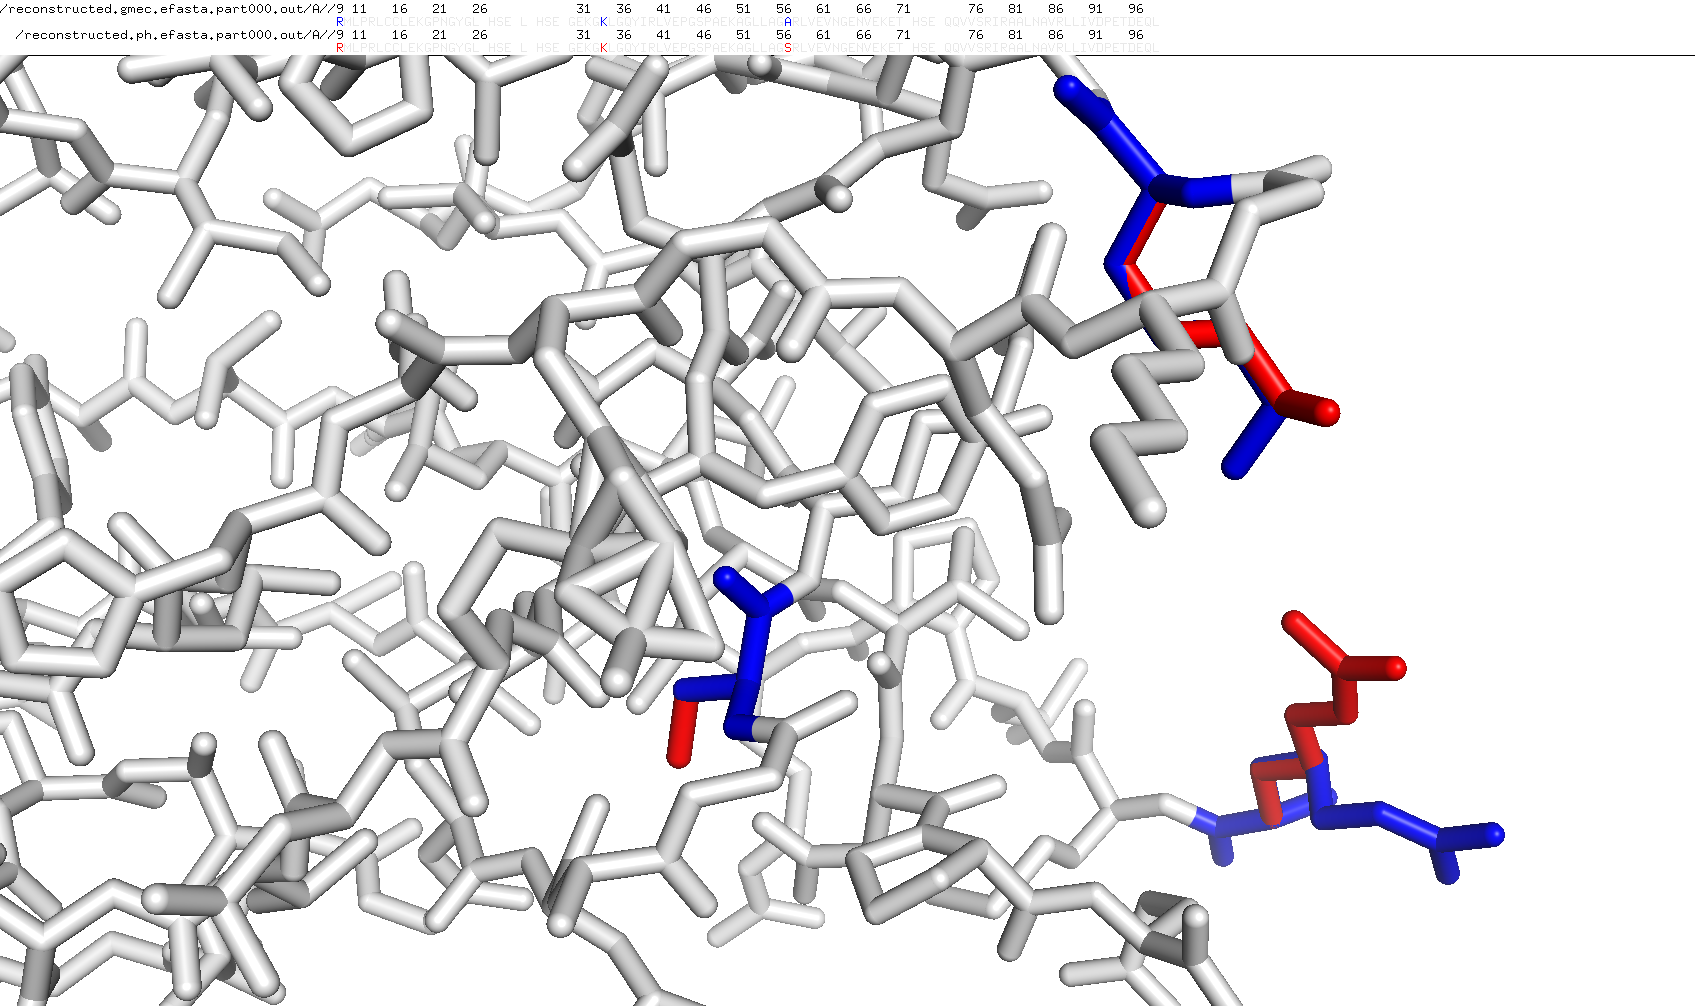
\includegraphics[width=14cm]{1G9O_3_gmec_vs_ph.png} 
      \end{tabular}
      
      \caption{test: 1G9O 3, GMEC vs H}
\label{image:1G9O_3_GMEC_vs_H}
    \end{figure}
    
    
    \begin{figure}[h]
      \centering
      \begin{tabular}{c} 
        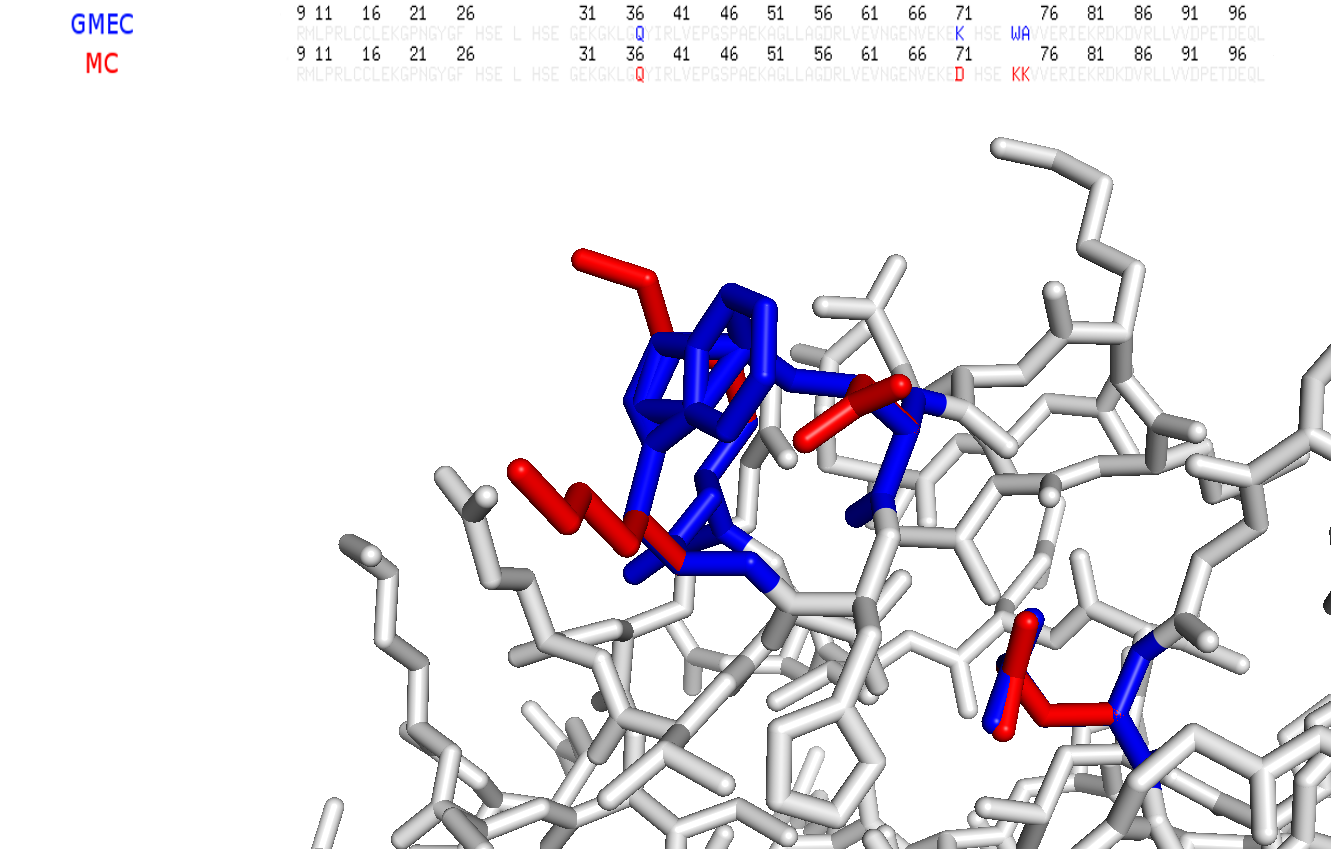
\includegraphics[width=14cm]{1G9O_5_gmec_vs_MC.png} 
      \end{tabular}
      
      \caption{test: 1G9O 5, GMEC vs MC}
\label{image:1G9O_5_GMEC_vs_MC}
    \end{figure}
    
    \begin{figure}[h]
      \centering
      \begin{tabular}{c} 
        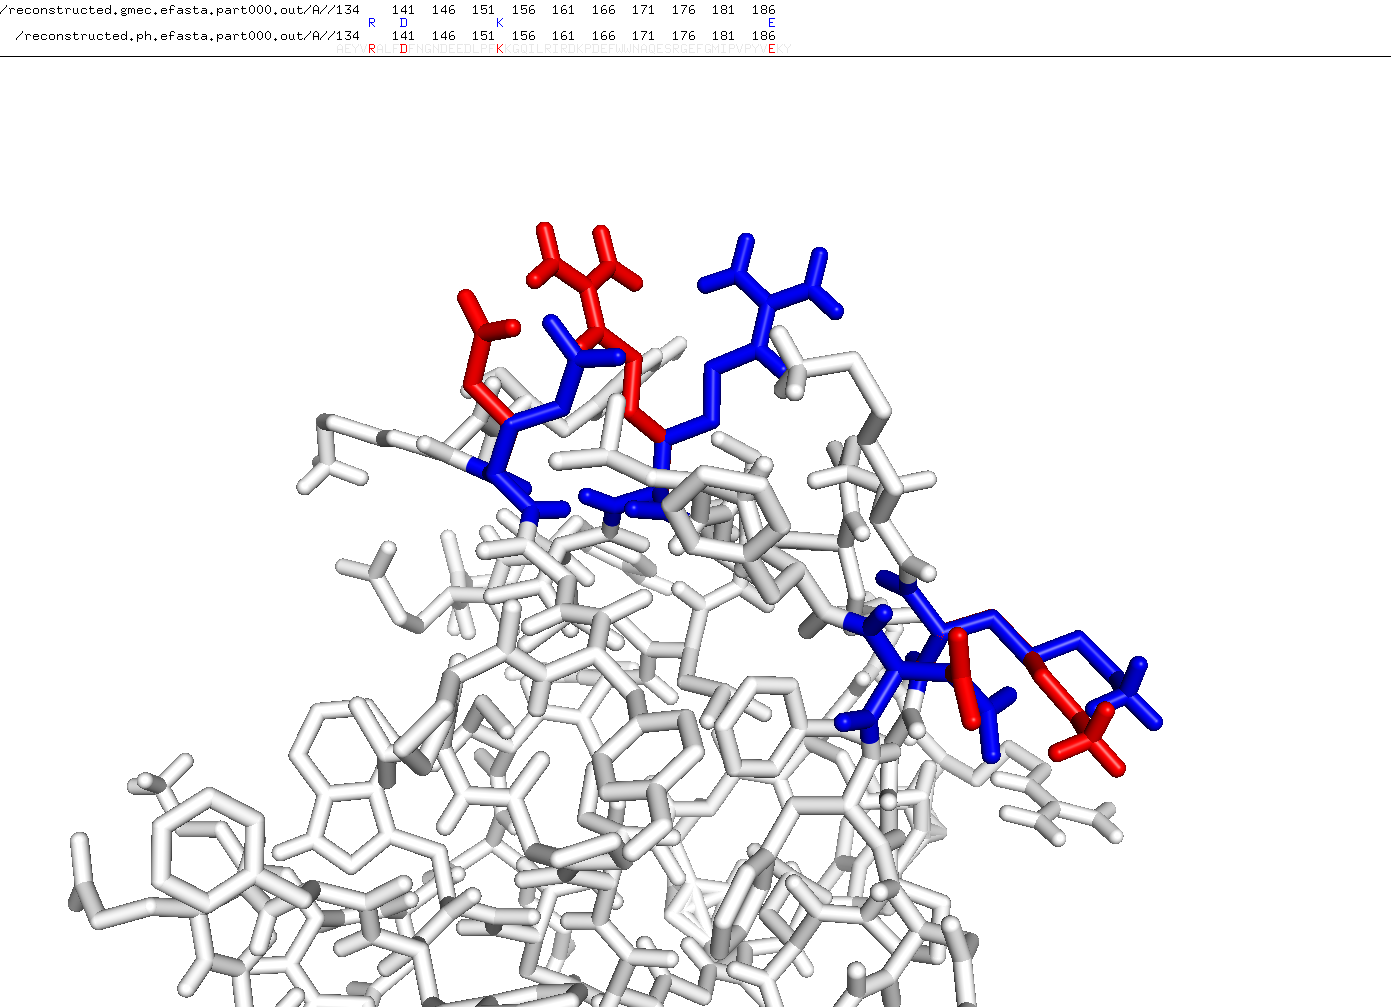
\includegraphics[width=14cm]{1CKA_5_gmec_vs_ph.png} 
      \end{tabular}
      
      \caption{test: 1CKA 5, GMEC vs H}
\label{image:1CKA_5_GMEC_vs_H}
    \end{figure}

    \begin{figure}[h]
      \centering
      \begin{tabular}{c} 
        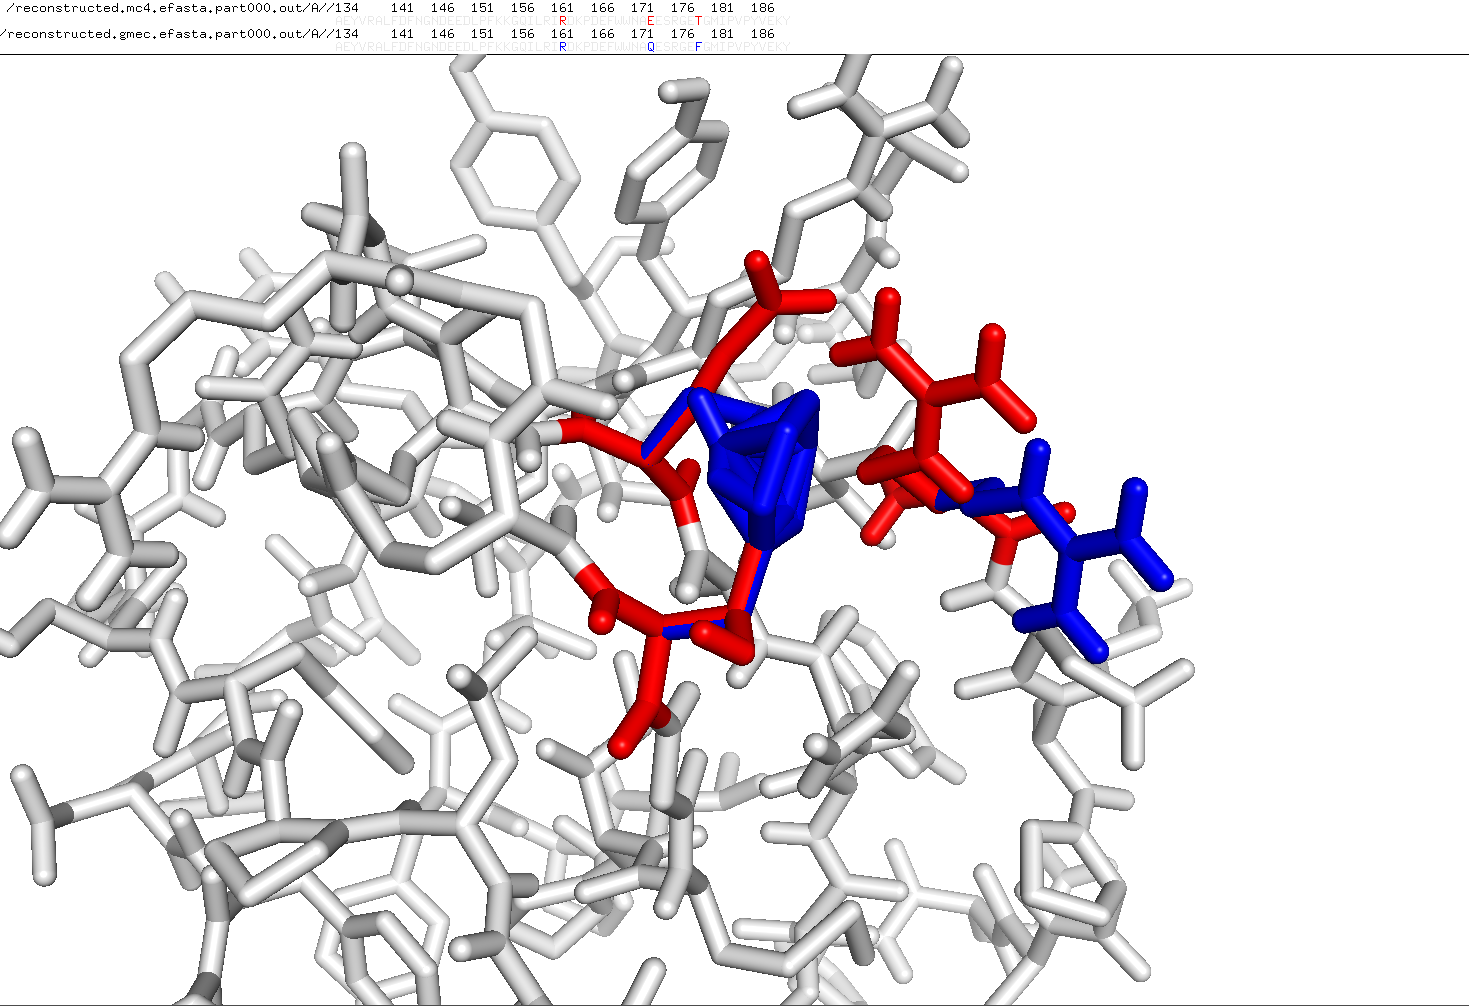
\includegraphics[width=14cm]{1CKA_5_gmec_vs_MC.png} 
      \end{tabular}
      
      \caption{test: 1CKA 5, GMEC vs MC}
\label{image:1CKA_5_GMEC_vs_MC}
    \end{figure}
    
    \clearpage


    \begin{figure}[h]
      \centering
      \begin{tabular}{c} 
        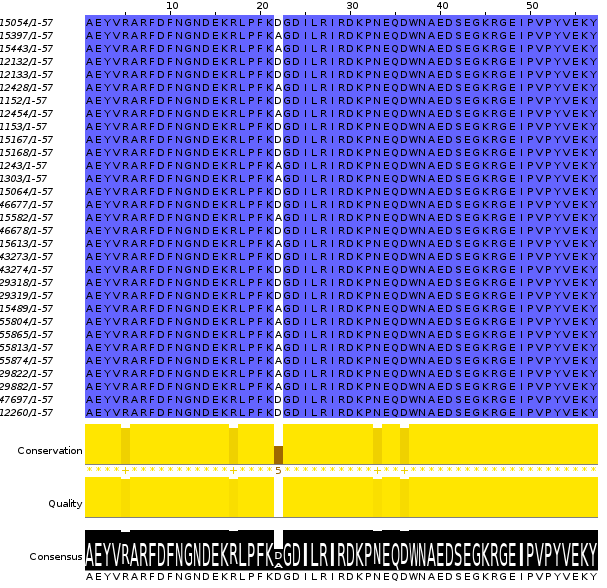
\includegraphics[width=14cm]{align_1CKA.png} 
      \end{tabular}
      
      \caption{Aligmenent du voisinnage: 1CKA 5}
\label{image:Align_Suboptimal}
    \end{figure}




   \subsection{Résultats Superfamily}


    \begin{table}[h]
           \raggedleft{}

      \begin{tabular}{cccccc}

        \toprule
        Protein & Match/seq size & Superfamily Evalue & superfamily success & Family Evalue & family success\\
        \cmidrule{1-6}
        1A81 & no & & & & \\
        1ABO & 51/58 & 4.4e-4 & 100\% & 2.8e-3 & 100\% \\
        1BM2 & 78/98 & 4.2e-5 & 100\% & 2.6e-3 & 100\% \\
        1CKA & 40/57 & 1.1e-5 & 100\% & 3.4e-3. & 100\% \\
        1G9O & 79/91 & 7.0e-7 & 100\% & 2.5e-3 & 100\%  \\
        1M61 & 97/109 & 7.2e-7 & 100\% & 2.6e-4 &  100\% \\
        1O4C & 95/104 & 2.1e-4 & 100\% & 4.5e-3 &  100\% \\
        1R6J & 74/82 & 9.8e-6 & 100\% & 4.6e-3 &  100\% \\
        2BYG & 59/97 & 1.4e-5 & 100\% & 7.1e-3 &  100\% \\
        \bottomrule        
      \end{tabular}      

\label{tab:superfamily_bestRE}       
\end{table}

    \clearpage



   \subsection{Résultats Heuristic (protocoles longs)}


    \begin{table}[h]
      \centering

      \begin{tabular}{ccccc}

        \toprule
        Proteins & GMEC & H & H+ & H++ \\
        \cmidrule{1-5}
        1ABO 1 & -309.1670 & -0.0675 & -0.0675 & 0 \\
        1CKA 5 & -299.2329 & -0.2859 & -0.0640 & 0 \\
        1G9O 3 & -477.2503 & -0.1366 & 0 & 0 \\
        1M61 2 & -538.6026 & -3.5105 & -2.1673 & -0.0188 \\
        \toprule


 \end{tabular}      
 \caption{Résultats pour 3 fois (resp 9 fois)plus de cycles heuristiques protocole H+ (resp H++)}
\label{tab:H+_H++}       
\end{table}


    \clearpage

   \subsection{densité en séquences }

    \begin{figure}[h]
      \centering
      \begin{tabular}{cc} 
        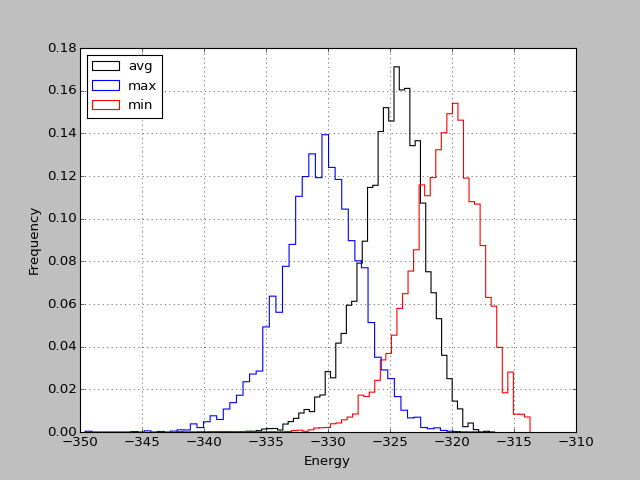
\includegraphics[width=10cm]{histo1_aa_Tambiante.png} &
      \end{tabular}
      
      \caption{.}
\label{graph:densité_en_séquences1}
    \end{figure}


    \begin{figure}[h]
      \centering
      \begin{tabular}{cc} 
        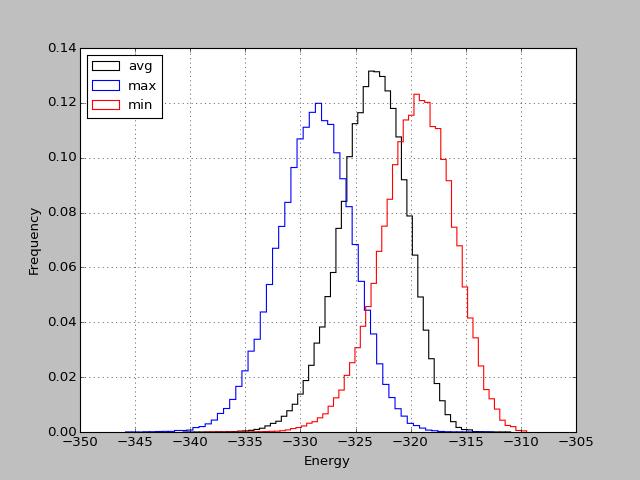
\includegraphics[width=10cm]{histo2_aa_Tambiante.png} &
      \end{tabular}
      
      \caption{.}
\label{graph:densité_en_séquences2}
    \end{figure}

    \clearpage




%%% Local Variables:
%%% mode: latex
%%% TeX-master: "../../rapport"
%%% End:
